%!TEX root=report.tex

\subsection{Tidsrækkeanalyse - SARIMA-model}

Da man for GRACE datasætte har mulighed for at se på et enkelt punkt og observere ændringerne i tyndekraften som en tidsserie,
virker det åbenlyst at forsøge at benytte en tidsrækkeanalyse model til at analysere dataen.
Det har dog vist sig ikke at være muligt, ihvertfald for de simple modeller brugt her.

Som udgangspunkt blev et punkt på Grøndlands kyst \todo{hvilket punkt} valg til at udforske mulighederne for en tidsrækkeanalyse.

Fælles for ARIMA modellerne er at den tidsrække man søger at modellere skal have equidistante tidsskridt,
ellers kan Yule-Walker ligningerne \cite[s.~122]{time-series-analysis} ikke løses.
I det oprindelige GRACE data er der manglende værdier - derfor anvendes splines \todo{kan ikke se hvordan splines, kan benyttes til interpolation her /A}
til at interpolere hen over de manglende observationer. Derefter tilsidesættes de sidste 12 observation som test data, til en krydsvalidering,
den resten del af tidsrækken er det som model bygges på.

\begin{figure}[H]
\centering
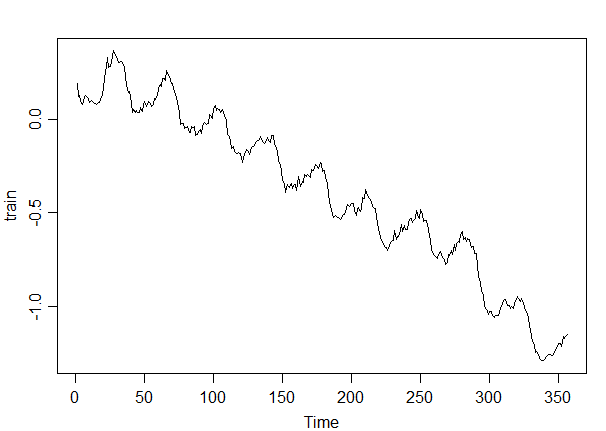
\includegraphics[height=4cm]{figures/yTrain}
\caption{GRACE data, hvor manglende data er udfyldt ved interpolation}
\label{fig:ts-y-train-raw}
\end{figure}

\begin{figure}[H]
\centering
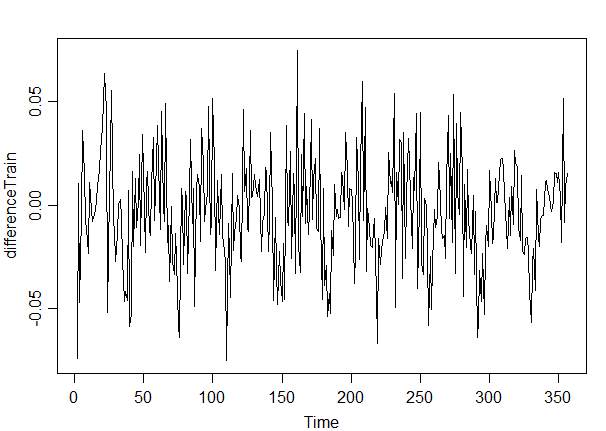
\includegraphics[height=4cm]{figures/differenceYTrain}
\caption{GRACE data, hvor manglende data er udfyldt ved interpolation}
\label{fig:ts-y-train-diff}
\end{figure}
Tidsrækken som ses i figur \ref{fig:ts-y-train-raw} ser periodisk ud men er ikke stationær.
Derfor undersøges differencen på serien, som er stationær (figur \ref{fig:ts-y-train-diff}).
Når man ser på differencen bliver det dog også tydeligt at tidsrække ikke er så pænt periodisk som man umiddelbart kunne have håbet på.

Her følger Auto korrelations funktionen og den partielle auto korrelations funktionen:
\begin{figure}[H]
	\centering
	\begin{subfigure}[b]{0.49\textwidth}
		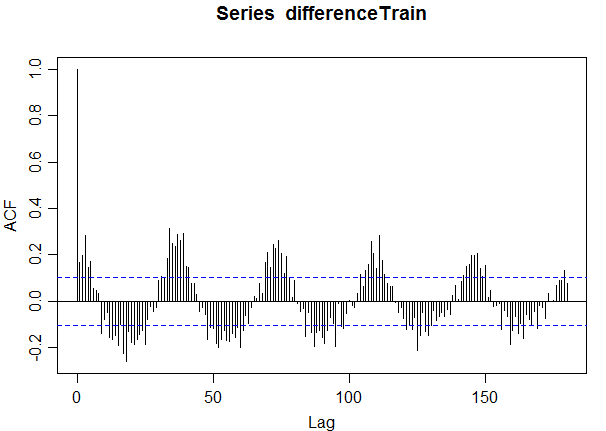
\includegraphics[width=\textwidth]{figures/acf}
		\caption{ACF til 5 års lag}
	\end{subfigure}
	\begin{subfigure}[b]{0.49\textwidth}
		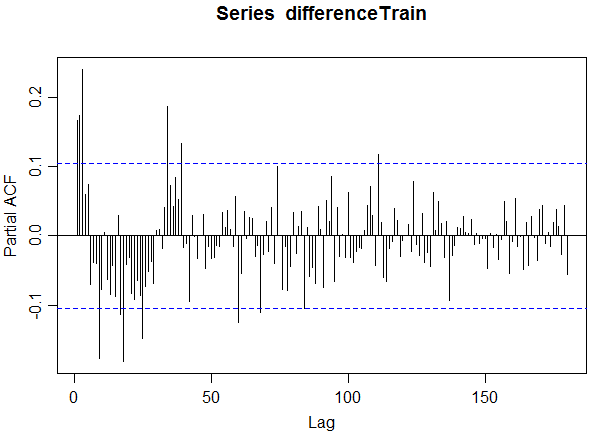
\includegraphics[width=\textwidth]{figures/pacf}
		\caption{PACF til 5 års lag}
	\end{subfigure}
	\caption{Viser kollerationen imellem residualerne på en \texttt{ARIMA(0,1,0)} model}
	\label{fig:ts-acf-pacf}
\end{figure}

I figur \ref{fig:ts-acf-pacf} ses at der ikke er specielt store korrelationer,
samtidig er de også rimelig konstante og derudover ligner det at afstanden mellem 2 toppe ikke er konstant
\todo{Jeg syntes den er pænt konstant i ACF, det at den er svær at se i PACF, indikere måske at der intet \texttt{SAR} led er. /A}
(der er ikke en klar sæson længde); alle disse faktorer  er indikatorer på at en ARIMA-model er et dårligt model valg.
Men hvis man skulle gøre et forsøg på at konstruere en model så siger teorien \cite[s.~155]{time-series-analysis} at:

\begin{itemize}
\item Ud fra ACF'en kan aflæses MA-led. Der er en peak på 3. lag, mens 4. og 5. lag er meget tæt på at være under signifikans grænsen -  dette kunne indikere op til MA(3)-led.
Ligeledes hvis man antager at funktionen er periodisk med svigninger per år, så kan man aflæse fra ACF'en at processen har op til SMA(4)-led.

\item Fra PACF-plottet kan AR-ledet aflæses. Med helt samme analoge metoder som ovenfor aflæses AR(3) og SAR(1) led.
Men igen, korrelationerne er endnu lavere i PACF'en end i ACF'en. 
\end{itemize}

Ud fra ovenstående estimeres en SARIMA model i R (Appendix \ref{first-R}) .
Mange af parametrene var dog ikke statistisk signifikant forskellige fra 0, de mindst vigtige parametre blev derfor iterativt fjernet, tilbage er følgende parametre:
\begin{lstlisting}
ARIMA(3,1,2)(0,1,1)[36]                    

Coefficients:
         ar1     ar2     ar3      ma1      ma2     sma1
      0.1292  0.4092  0.1346  -0.3020  -0.5008  -0.7601
s.e.  0.3551  0.2545  0.0653   0.3562   0.2860   0.0641
\end{lstlisting}

\begin{figure}[H]
\centering
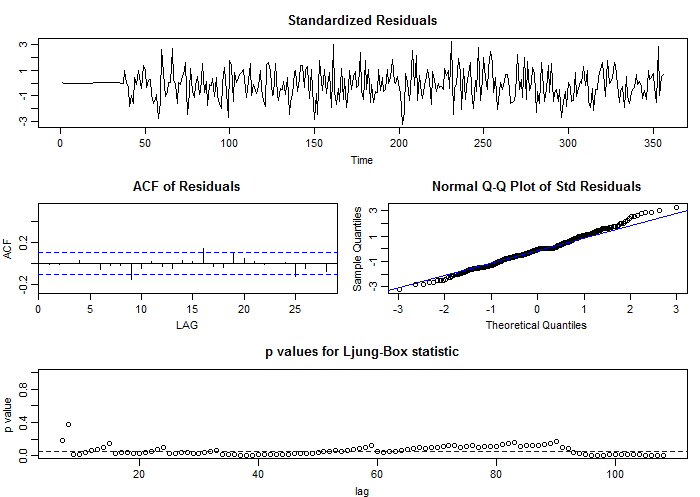
\includegraphics[width=\textwidth]{figures/tsDiagnostics}
\caption{Diagnose af residualerne på en SARIMA $(3,1,2) \times (0,1,1)_{36}$ model.}
\label{fig:ts-tsdiag}
\end{figure}
Som det ses i figur \ref{fig:ts-tsdiag} er residualerne ikke specielt imponerende.
Selvom ACF, og QQ-plottet ser fornuftigt ud så kan man i Ljung-Box plottet se at det for mange lags kan statistisk afvises at residualerne er hvid støj.
Dette indikerer stærk at der er ydeligere mønstre, som ikke er er fanget af denne SARIMA model.
Dermed er det lidt misvise at prøve at predikter eller fortolke på modellen,
men for komplethedens skyld skyld udregnes 12-step ahead prædiktioner og disse sammenlignes med test dataen:

\begin{figure}[H]
\centering
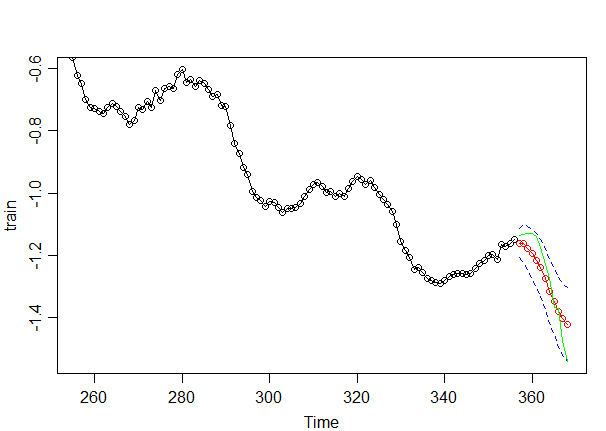
\includegraphics[height=6cm]{figures/tsPredictions}
\caption{Trænings data i sort, predictions i rød, 95\%-konfidens interval i blå og test data i grøn.}
\label{fig:ts-crossvalidate}
\end{figure}

Af figur \ref{fig:ts-crossvalidate} ses det at test observationerne rent faktisk holder sig inden for 95\% konfidensintervallet,
men det ses samtidig at mønstret/bevægelsen er meget anderledes fra den predikterede bevægelse.

Man kan konkludere at modellen ikke er praktisk anvendelig.
Hvis man ville bruge mere tid på det forventer vi dog at man kunne opnå bedre resultater med exogene variabler så som regnmængde
\todo{men det er jo bl.a. det vi prøver at udtale os om, så anden data giver ikke mening. /A} og temperatur,altså en SARIMAX model.
